%% MQ-11-66-sorcerer
\section{Sorcerer}
\label{monster:sorcerer}


\includegraphics[height=2cm,keepaspectratio]{./resources/monster/sorcerer}

\begin{longtable}{ l p{9cm} }
	HP
	& 840
\\ \hline
	Exp
	& 627
\\ \hline
	GP
	& 21
\\ \hline
	Strategy
	& Heavy magic users. \textit{Quake}, in particular, can do some fair damage on your characters. \\
	& They lack defense though. Take them out in one or two attacks. \\
	& Make sure not to leave them only half-dead though, they can cure themselves.
\\ \hline
	Weakness
	& 
\includegraphics[height=1em,keepaspectratio]{./resources/effects/shoot} Shoot \\
	& 
\includegraphics[height=1em,keepaspectratio]{./resources/effects/wind} Wind
\\ \hline
	Resist
	& 
\includegraphics[height=1em,keepaspectratio]{./resources/effects/earth} Earth
\\ \hline
	Abilities
	& 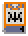
\includegraphics[height=1em,keepaspectratio]{./resources/spells/cure} Cure \\
	& 
\includegraphics[height=1em,keepaspectratio]{./resources/effects/water} Blizzard \\
	& 
\includegraphics[height=1em,keepaspectratio]{./resources/effects/earth} Earth \\
	& 
\includegraphics[height=1em,keepaspectratio]{./resources/effects/silence} Muffle \\
	& 
\includegraphics[height=1em,keepaspectratio]{./resources/effects/wind} Thunder
\end{longtable}
